\newcommand{\DoNotLoadEpstopdf}{}
\documentclass[11pt]{article}
\usepackage[T1]{fontenc}
\usepackage[utf8]{inputenc}
\usepackage{lmodern}
\usepackage[margin=1.05in]{geometry}
\usepackage{amsmath,amssymb,amsthm,mathtools}
\usepackage{microtype,enumitem,booktabs,array,float}
\usepackage{tikz}
\usetikzlibrary{arrows.meta,calc,patterns,positioning}
\usepackage[numbers,sort&compress]{natbib}
\usepackage{xurl}
\usepackage[colorlinks=true,linkcolor=blue!45!black,citecolor=blue!45!black,urlcolor=blue!45!black]{hyperref}
\hypersetup{pdftitle={Maximal Multipoint Seshadri Constants in Higher Dimensions},pdfauthor={OpenAI}}
\ifdefined\pdfinfoomitdate\pdfinfoomitdate=1\fi
\ifdefined\pdftrailerid\pdftrailerid{}\fi
\ifdefined\pdfsuppressptexinfo\pdfsuppressptexinfo=15\fi
\setlength{\emergencystretch}{1em}
\setlength{\parskip}{0.1em}
\numberwithin{equation}{section}
\newtheorem{theorem}{Theorem}[section]
\newtheorem{proposition}[theorem]{Proposition}
\newtheorem{lemma}[theorem]{Lemma}
\newtheorem{corollary}[theorem]{Corollary}
\theoremstyle{definition}
\newtheorem{definition}[theorem]{Definition}
\newtheorem{remark}[theorem]{Remark}
\newcommand{\C}{\mathbb C}
\newcommand{\R}{\mathbb R}
\newcommand{\Z}{\mathbb Z}
\newcommand{\N}{\mathbb N}
\newcommand{\Torus}{\mathbb T}
\newcommand{\M}{\mathcal M}
\newcommand{\Jet}{\mathrm J}
\newcommand{\eps}{\varepsilon}
\newcommand{\frakm}{\mathfrak m}
\DeclareMathOperator{\vol}{vol}
\DeclareMathOperator{\conv}{conv}
\DeclareMathOperator{\ord}{ord}
\DeclareMathOperator{\mult}{mult}
\DeclareMathOperator{\Span}{span}
\DeclareMathOperator{\length}{length}
\DeclareMathOperator{\Supp}{Supp}
\title{Maximal Multipoint Seshadri Constants\protect\\ in Higher Dimensions}
\author{OpenAI}
\date{October 5, 2026}
\begin{document}
\maketitle
\begin{abstract}
Let $L$ be an ample line bundle on a smooth integral complex projective variety
$X$ of dimension $n\ge3$. We prove that there is a threshold
$r_0=r_0(X,L)$ such that for every integer $r\ge r_0$, the ordinary multipoint
Seshadri constant at $r$ very general points equals the volume bound
$(L^n/r)^{1/n}$. This establishes the qualitative Nagata--Biran--Szemberg
assertion in these dimensions.
\end{abstract}
\section{Introduction}\label{sec:introduction}

Let $X$ be a smooth integral complex projective variety of dimension $n\ge3$,
and let $L$ be an ample line bundle. Put $V=L^n$. For a tuple
$\mathbf p=(p_1,\ldots,p_r)$ of distinct points, the ordinary multipoint
Seshadri constant is
\begin{equation}\label{eq:seshadri-definition}
 \eps(X,L;\mathbf p)
 =\inf_C\frac{L\cdot C}{\sum_{i=1}^r\mult_{p_i}C},
\end{equation}
where $C$ ranges over integral curves meeting at least one of the marked
points, and the multiplicity is zero at points outside $C$. This invariant
measures the local positivity of $L$ at the entire tuple. Its universal
upper bound is
\begin{equation}\label{eq:volume-bound}
 \eps(X,L;\mathbf p)\le (V/r)^{1/n}.
\end{equation}
Equality means that no curve imposes a stronger constraint than the volume
of $L$.

Write
\[
 U_r(X)=\{(p_1,\ldots,p_r)\in X^r:p_i\ne p_j\text{ when }i\ne j\}.
\]
A property holds at \emph{very general} tuples if the exceptional tuples
are contained in a countable union of proper Zariski-closed subsets of
$U_r(X)$.

\begin{theorem}\label{thm:main}
Let $X$ be a smooth integral complex projective variety of dimension
$n\ge3$, and let $L$ be an ample line bundle on $X$. There is an integer
$r_0=r_0(X,L)\ge1$ such that for every integer $r\ge r_0$ there is a
countable union $Z_r$ of proper Zariski-closed subsets of $U_r(X)$, with
nonempty complement, for which
\[
 \eps(X,L;\mathbf p)=\left(\frac{L^n}{r}\right)^{1/n}
 \qquad\text{for every }\mathbf p\in U_r(X)\setminus Z_r.
\]
\end{theorem}

\begin{samepage}
Equivalently, on the blow-up $\pi:Y\to X$ at such a tuple, with exceptional
divisors $E_1,\ldots,E_r$, the real divisor class
\[
 \pi^*L-(V/r)^{1/n}\sum_{i=1}^rE_i
\]
is nef and has top self-intersection zero. Here nefness means nonnegative
intersection with every integral curve. The threshold depends on the fixed
polarized variety, but all integers beyond it are included. In particular,
Theorem~\ref{thm:main} asserts exact equality for each such point count,
rather than convergence of a normalized constant as $r$ increases.
\end{samepage}

\subsection{Background and relation to earlier work}

The plane problem originates in Nagata's work on Hilbert's fourteenth
problem. He conjectured a lower bound on the degree of a plane curve in
terms of its multiplicities at very general points, and proved the strict
inequality when the number of points is a square at least $16$
\cite{Nagata1959}. Multipoint Seshadri constants express the corresponding
positivity question on an arbitrary polarized variety. The qualitative
Nagata--Biran--Szemberg formulation asks for maximality at every sufficiently
large point count. Ro\'e and Ross state this formulation in arbitrary
dimension and distinguish the ordinary curve-defined constant from its
higher-cycle analogues \cite[Conjecture~1.3 and Remark~1.4]{RoeRoss2009}.
We use the ordinary constant throughout, even when $\dim X>2$.

Biran's packing stability theorem supplies an important symplectic
precedent: sufficiently many equal balls can fill a closed symplectic
four-manifold with rational symplectic class with arbitrarily small volume
deficit \cite{Biran1999}; see also \cite[Theorem~6.3]{Biran2001}. The algebraic
question fixes the complex variety and asks for a nef class on its point
blow-ups, so symplectic packing stability is not by itself the required
algebraic statement. In arbitrary dimension, K\"uchle obtained lower bounds
for multipoint Seshadri constants that are asymptotically optimal as the
number of points tends to infinity \cite[Theorem~1.1]{Kuechle1996}.
Biran's product inequality, extended to higher-cycle constants by
Ro\'e--Ross, relates point counts on a variety to point counts on projective
space \cite[Theorem~1.1 and Remark~1.2]{RoeRoss2009}.
These results illuminate the volume scale in \eqref{eq:volume-bound}; an
asymptotically optimal estimate alone does not imply eventual equality.

The companion paper \cite{OpenAI2026Surfaces} establishes the qualitative
surface statement by a nodal exponent bound, diagonal slice compression,
and a primitive lattice direction tuned to the number of points. Its final
tests are \emph{injective} jet evaluations on finite torus subgroups.
We adapt the planar geometric mechanism to polynomial spaces in two
variables and use \emph{surjective} full-dimensional jet evaluations instead.
All arguments required for this adaptation are proved here; the surface
maximality theorem is not an input.

The interpretation of positivity through asymptotic jet generation is
classical; see Demailly \cite[Section~6]{Demailly1992}.
Our use of initial monomials belongs to the valuation approach to linear
series initiated by Okounkov \cite{Okounkov1996} and developed by Lazarsfeld--Musta\c{t}\u{a}
\cite{LazarsfeldMustata2009} and Kaveh--Khovanskii
\cite{KavehKhovanskii2012}. More directly, Ito compares multipoint jet
separation with initial monomial spaces by separate finite-degree
degenerations, without a finite-generation hypothesis
\cite[Proposition~5.7 and Theorem~5.8]{Ito2013}.
Monomial diagrams and interpolation minors also underlie Dumnicki's
diagram-cutting method \cite[Proposition~13 and Theorem~14]{Dumnicki2007}.
We retain elementary proofs of the specific transfer and counting statements
used below.

\subsection{Proof strategy and the two-coordinate construction}

Separating jets through degree $m$ at a tuple means prescribing,
independently at each point, all Taylor coefficients of total degree at
most $m$, in local coordinates and line-bundle frames. If $H^0(X,kL)$
separates these jets, then
\[
 \eps(X,L;\mathbf p)\ge \frac{m}{k};
\]
the curve-intersection argument is given in Lemma~\ref{lem:jets-curves}.
Thus, for $w=(V/r)^{1/n}$, our interpolation target is jet separation
through degree $\lfloor k\theta\rfloor$ for every fixed $0<\theta<w$
and all sufficiently large $k$. We first construct a tuple for each such
test and later obtain simultaneous tests at very general tuples.

The argument works with finite exponent sets
$S_k\subset\Z^n$, one for each positive integer degree $k$, satisfying
\[
 S_k+S_l\subset S_{k+l}.
\]
For a set $S$, its monomial space is the span of the Laurent monomials
$z^\alpha$ with $\alpha\in S$ on $(\C^*)^n$. The multiplication condition
will be as important as the geometry of the individual sets.

A complete-intersection flag on $X$ first supplies sets $S_k$ whose
cardinalities are $h^0(X,kL)$. They lie in the dilates of a simplex
\[
 \Delta(a_1,\ldots,a_n)
 =\left\{x\in\R_{\ge0}^n:\sum_{i=1}^n\frac{x_i}{a_i}\le1\right\}
\]
of volume $V/n!$. Jet surjectivity for the corresponding monomials can be
transferred back to sections on $X$.

The main construction replaces any two intercepts $A,B$ of the bounding
simplex by $w,AB/w$, for any sufficiently small positive real $w$.
It preserves the number of exponents, the multiplication condition, and
the implication from jet surjectivity after the replacement to jet
surjectivity before it. The other exponent coordinates are carried along
unchanged. The planar node bound and primitive-direction argument come
from the surface method; the real-intercept replacement and its compatibility
with these remaining coordinates allow the process to be iterated in
higher dimensions.

For a fixed sufficiently large integer $r$, choose $w=(V/r)^{1/n}$.
Repeated replacements produce sets $F_k$ inside dilates of
\[
 P_* = \Delta(w,\ldots,w,rw),
 \qquad \#F_k=h^0(X,kL),
 \qquad F_k+F_l\subset F_{k+l}.
\]
Because this simplex still has volume $V/n!$, only $o(k^n)$ of its degree-$k$
lattice points are missing. The multiplication condition upgrades this
density statement: for each fixed compact set $K\subset\operatorname{int}P_*$,
every lattice point of $kK$ belongs to $F_k$ for all sufficiently large $k$.
Indeed, such a point has on the order of
$k^n$ decompositions into two nearly equal degrees, whereas the holes can
exclude only $o(k^n)$ of them. This short argument is a full-density version
of the interior approximation results for semigroups
\cite[Theorem~1.6]{KavehKhovanskii2012}.

The long last intercept of $P_*$ permits explicit interpolation at $r$
points that differ only in their last coordinate. One-variable Hermite
interpolation, applied to the coefficients of monomials in the other
coordinates, gives arbitrary jets through degree $\lfloor k\theta\rfloor$
for every fixed $0<\theta<w$ and all sufficiently large $k$.
Transferring these tests to $X$, taking a countable intersection of
nonempty Zariski-open loci, and then letting $\theta$ increase to $w$
proves Theorem~\ref{thm:main}.

Section~\ref{sec:transfers} establishes the monomial operations and their
jet transfers, and Section~\ref{sec:flag} constructs the initial exponent
sets on $X$. Section~\ref{sec:reshaping} proves the two-coordinate
replacement. Section~\ref{sec:saturation} establishes interior filling and
interpolation, and Section~\ref{sec:conclusion} assembles the very-general
conclusion.

\section{Monomial spaces and finite jets}
\label{sec:transfers}

The proof will replace spaces of sections by monomial spaces and then change
their exponent sets. Two properties must survive these changes: multiplication
between different degrees, and the implication that interpolation for the new
space yields interpolation for the old one. We establish these properties
separately. Multiplication concerns the exact exponent sets in every degree;
interpolation will be transferred by analytic limits at one fixed degree.

\subsection{Jets and graded exponent sets}

Write $\Torus^n=(\C^*)^n$. For a finite set $S\subset\Z^n$, put
\[
 \M(S)=\Span_{\C}\{x^\alpha:\alpha\in S\},
 \qquad x^\alpha=x_1^{\alpha_1}\cdots x_n^{\alpha_n}.
\]
These Laurent polynomials are regular on $\Torus^n$. If $A$ is a line bundle
on a smooth complex variety $Y$, its jets through an integer degree $m\geq0$ at $p\in Y$
form the vector space
\[
 \Jet_p^m(A)
 =A_p/\frakm_p^{m+1}A_p.
\]
Here $A_p$ denotes the stalk of the sheaf of sections. A space of sections
$W$ \emph{separates jets through degree $m$} at distinct points
$p_1,\ldots,p_r$ if the evaluation map
\[
 W\longrightarrow\bigoplus_{i=1}^r\Jet_{p_i}^m(A)
\]
is surjective. For functions we use the trivial line bundle. Local frames and
local coordinates change the matrices of these maps but not their ranks.
Analytic and algebraic finite jets agree at a smooth complex point, since
the corresponding local rings have the same completion.
Our aim is to obtain such surjections for $W=H^0(X,kL)$ with $m/k$
approaching $(V/r)^{1/n}$.

\begin{definition}\label{def:graded-support}
A \emph{graded support family} in $\Z^n$ is a sequence of finite sets
$(S_k)_{k\geq1}$ such that
\begin{equation}\label{eq:graded-support}
 S_k+S_l\subset S_{k+l}\qquad(k,l\geq1).
\end{equation}
Empty sets are allowed. Equivalently,
$\M(S_k)\M(S_l)\subset\M(S_{k+l})$, where a product of spaces denotes the
span of their pairwise products.
\end{definition}

We will say that an operation on monomial spaces \emph{transfers jet
separation backward} if, for every fixed degree, number of points, and jet
order, separation by the output space at some distinct torus tuple implies
separation by the input space at some distinct torus tuple. The tuples need
not be the same. A finite sequence of such operations has the same property.

\subsection{Least terms and analytic limits}

A monomial order on $\Z_{\geq0}^q$ will mean a total well-order preserved by
addition. For a nonzero convergent power series $f$, let $\nu(f)$ be the
least exponent in its support for this order.

\begin{lemma}[Least-term bases]\label{lem:least-terms}
Let $W$ be a finite-dimensional space of convergent power series in $q$
variables, and fix a monomial order. The set
\[
 \nu(W\setminus\{0\})
\]
has cardinality $\dim W$. There is a basis of $W$ whose least exponents are
exactly this set, with each least coefficient equal to $1$. Moreover,
$\nu(fg)=\nu(f)+\nu(g)$ for nonzero convergent power series $f,g$.
\end{lemma}

\begin{proof}
If $W\ne0$, choose the smallest exponent occurring as the least exponent of
an element of $W$, and normalize one such element to have coefficient $1$
there. Continue in the kernel of that coefficient functional, which has
codimension one. After $\dim W$ steps this gives a basis with strictly
increasing least exponents. In any nonzero linear combination, the first
basis element with a nonzero coefficient determines the least term. This
proves the assertion about the whole set of possible exponents.

For the product assertion, write $a=\nu(f)$ and $b=\nu(g)$. Every exponent
of $f$ is at least $a$, and every exponent of $g$ is at least $b$. Additivity
of the order implies that any pair other than $(a,b)$ has sum strictly
greater than $a+b$. The coefficient of $x^{a+b}$ in the product is therefore
the product of the two nonzero least coefficients.
\end{proof}

\begin{lemma}[Least terms in labeled spaces]\label{lem:row-valuation}
Fix integers $1\leq q\leq n$ and a monomial order in $q$ variables. For
$k\geq1$ and $\gamma\in\Z^{n-q}$, let $W_{k,\gamma}$ be
finite-dimensional spaces of convergent power series in those variables,
with only finitely many nonzero spaces in each degree. Assume that
\[
 W_{k,\gamma}W_{l,\eta}\subset W_{k+l,\gamma+\eta}
 \qquad(k,l\geq1;\ \gamma,\eta\in\Z^{n-q}).
\]
Then
\[
 S'_k=\{(\nu(f),\gamma):0\ne f\in W_{k,\gamma}\}
\]
is a graded support family and
$\#S'_k=\sum_\gamma\dim W_{k,\gamma}$.
\end{lemma}

\begin{proof}
The cardinality assertion follows from Lemma~\ref{lem:least-terms} in each
label. Given two exponents in $S'_k$ and $S'_l$, choose functions witnessing
them. Their nonzero product belongs to the summed degree and label, and
its least exponent is the sum of the two least exponents.
Expanding products of arbitrary linear combinations therefore gives
$\M(S'_k)\M(S'_l)\subset\M(S'_{k+l})$. The full new monomial spaces
thus retain the multiplication property needed for the next operation;
no simultaneous choice of lifts to earlier spaces is required.
\end{proof}

The finite-degree passage to initial monomials is a standard
jet-degeneration principle; see \citet[Proposition~5.7]{Ito2013}. The next
two lemmas give the direct analytic form used here, including unchanged
coordinate factors. The first is analytic; the second is finite-dimensional
linear algebra.

\begin{lemma}[Weighted limits with unchanged variables]
\label{lem:weighted-limit}
Let $1\leq q\leq n$, and let $f_1,\ldots,f_N$ be convergent power series
near $0\in\C^q$. Suppose
that a vector $\lambda\in\R_{>0}^q$ makes a specified exponent $e_j$ the
unique minimum of $\lambda\cdot\alpha$ on the support of $f_j$, and let
$c_j\ne0$ be its coefficient. For any
$\gamma_j\in\Z^{n-q}$, as $s\downarrow0$ the functions
\begin{equation}\label{eq:weighted-limit}
 c_j^{-1}s^{-\lambda\cdot e_j}
 f_j(s^{\lambda_1}Z_1,\ldots,s^{\lambda_q}Z_q)U^{\gamma_j}
 \longrightarrow Z^{e_j}U^{\gamma_j}
\end{equation}
converge locally uniformly on $\C^q\times\Torus^{n-q}$, with all derivatives
of any fixed finite order. The assertion means that each fixed compact set
is in the domain of the left-hand side for all sufficiently small $s>0$.
When $q=n$, the unchanged variable block is omitted.
\end{lemma}

\begin{proof}
First omit the unchanged factor $U^{\gamma_j}$. On a bounded polydisc in
$Z$, choose $s_0>0$ small enough that the power series converges absolutely
on a slightly larger polydisc after scaling by $s_0^\lambda$. In the
normalized expansion every exponent $\lambda\cdot(\alpha-e_j)$ is
nonnegative, and every exponent other than the least one is strictly
positive. For $0<s\leq s_0$, the terms are
dominated by the summable series obtained at $s_0$. Dominated convergence
gives locally uniform convergence to $Z^{e_j}$. Applying Cauchy's estimates
on slightly larger polydiscs gives convergence of derivatives. The unchanged
Laurent monomials and their derivatives are holomorphic near every compact
subset of the torus, so multiplying by them preserves these conclusions.
\end{proof}

\begin{lemma}[Persistence of jet separation]\label{lem:rank-transfer}
Fix a finite tuple of distinct points in a complex manifold and a jet order
$m$. Suppose that finitely many holomorphic functions, depending on a
positive parameter $s$, converge with their derivatives through order $m$
near that tuple. If the limiting functions separate those jets, then the
functions for sufficiently small $s>0$ do also.

The same conclusion applies to sections written in local frames. If the
functions before the limit are pullbacks under a coordinate change sending
the tuple to distinct points, their original functions separate jets at the
image tuple. Multiplication of individual functions by nonzero constants
does not affect this statement.
\end{lemma}

\begin{proof}
Choose coordinates and frames near the points. The entries of the jet matrix
are the finitely many required Taylor coefficients. A maximal minor that is
nonzero in the limit remains nonzero for small $s$. Coordinate changes and
frame changes induce isomorphisms of truncated local rings or their
rank-one modules. Rescaling an individual function rescales a matrix column
by a nonzero constant.
\end{proof}

In particular, the unchanged variables in
Lemma~\ref{lem:weighted-limit} cause no restriction on the jets being
separated: all derivatives, including derivatives in those variables, enter
the same convergent jet matrix. We shall apply the lemmas to finitely many
spaces distinguished by a common exponent in the unchanged variables.

\subsection{Lattice changes and coordinate compression}

We next record two operations directly on Laurent monomials. They will let
us change the shape of an exponent set while retaining both properties
above.

\begin{lemma}[Unimodular changes]\label{lem:unimodular}
Let $B\in\operatorname{GL}_n(\Z)$. Replacing $S_k$ by $BS_k$ preserves
cardinality and the graded support property. It preserves, in both
directions, the existence of a distinct torus tuple at which the associated
monomial space separates any prescribed finite jets.
\end{lemma}

\begin{proof}
The lattice map is bijective and additive. The torus automorphism
\[
 \phi_B(x)_j=\prod_{i=1}^n x_i^{B_{ij}}
\]
has pullback $\phi_B^*(x^\alpha)=x^{B\alpha}$. Its inverse is the
monomial map associated with $B^{-1}\in\operatorname{GL}_n(\Z)$, so the
jet assertion follows by change of coordinates.
\end{proof}

For compression in the first coordinate, write an exponent as $(a,\beta)$
with $a\in\Z$ and $\beta\in\Z^{n-1}$. For a finite set $S$, define its
row space at $\beta$ by
\[
 W_\beta(S)=\Span_\C\{z^a:(a,\beta)\in S\},
\]
and define the compressed exponent set by
\begin{equation}\label{eq:coordinate-compression}
 \mathcal C_1(S)=
 \{(\ord_{z=1}f,\beta):0\ne f\in W_\beta(S)\}.
\end{equation}
All functions in a row are holomorphic near $z=1$, even when their
exponents are negative. Compression in another coordinate is defined by
permuting coordinates.

\begin{lemma}[Coordinate compression]\label{lem:compression}
Coordinate compression preserves the cardinalities and the graded support
property of a family $(S_k)$. It transfers jet separation backward. In a
nonempty row with smallest and largest exponents $a_-$ and $a_+$, every
compressed exponent lies in $[0,a_+-a_-]$.

Consequently, suppose that, after fixing all but two coordinates, the pair
exponents lie in a scaled convex polygon $\kappa Q$, where $\kappa\geq0$.
Compression in one pair coordinate bounds the new pair exponents by the
shape obtained by moving each interval slice parallel to that coordinate
to start at zero, without changing its length. This shape operation commutes
with scaling by $\kappa$.
\end{lemma}

\begin{proof}
Use the coordinate $u=z-1$ near $z=1$. Lemma~\ref{lem:least-terms}
identifies the possible orders in a row with a basis of distinct leading
orders. If the input sets are graded, the product of two row spaces lies in
the summed degree and remaining exponent. Lemma~\ref{lem:row-valuation}
therefore proves both cardinality preservation and the graded support
property.

Multiplying a nonzero row element by the unit $z^{-a_-}$ gives a polynomial
of degree at most $a_+-a_-$. Its order at $1$ is unchanged and cannot exceed
that degree. This proves the row bound, including for Laurent exponents.

For a fixed degree, choose in every nonempty row a basis with distinct
orders and leading coefficients $1$ in $u$. Substitute $z=1+sZ$, normalize
each basis element by $s$ to its order, and carry along the unchanged
monomial in the other variables. Lemmas~\ref{lem:weighted-limit}
and~\ref{lem:rank-transfer} apply to all rows simultaneously. At a fixed
finite torus tuple, the substitution has nonzero values and is injective
for sufficiently small $s>0$. It gives a local coordinate change, so jet
separation transfers to the original space at the image tuple.

Finally, a row contained in an interval slice of $\kappa Q$ has exponent
span no greater than the length of that slice. Its compressed row is
therefore contained in the interval beginning at zero with that length.
For $\kappa>0$, slices and their lengths scale by $\kappa$. When
$\kappa=0$, the only possible pair exponent is zero and compression leaves
it unchanged.
\end{proof}

When these operations act on a graded family, the support sets are defined
by fixed exact orders and fixed lattice maps. The weights and small
parameters used to transfer jets may nevertheless depend on the degree:
they only establish finite-rank implications. The multiplication property
in Lemma~\ref{lem:row-valuation} holds independently of those analytic
choices.

\section{A simplex from a complete-intersection flag}
\label{sec:flag}

We now associate to $(X,L)$ a graded support family with the same dimensions
as the spaces of sections. Its exponent sets lie in a simplex whose volume
is exactly the leading coefficient of the Hilbert polynomial. This equality
of volumes will later ensure that changing the shape of the simplex loses
no asymptotic supply of exponents.

Encoding sections by the least exponents associated with a flag is standard
in the theory of Okounkov bodies; see, for example,
\citet[Lemma~1.3]{LazarsfeldMustata2009}. For our complete-intersection flag,
the required bound follows directly from division by its defining sections
and a degree calculation on the final curve.

For positive real numbers $a_1,\ldots,a_n$, write
\begin{equation}\label{eq:simplex-definition}
 \Delta(a_1,\ldots,a_n)
 =\left\{y\in\R_{\geq0}^n:
              \sum_{i=1}^n\frac{y_i}{a_i}\leq1\right\}.
\end{equation}
Its Euclidean volume is $a_1\cdots a_n/n!$.

\begin{proposition}[The initial simplex]\label{prop:flag-simplex}
Let $X$ be a smooth integral complex projective variety of dimension
$n\geq3$, let $L$ be ample, and put $V=L^n$. Choose a positive integer $D$
such that $DL$ is very ample. There is a graded support family
$S_k\subset\Z_{\geq0}^n$ such that
\begin{align}
 S_k&\subset kP_0,
 &P_0&=\Delta(1/D,\ldots,1/D,D^{n-1}V),
 \label{eq:flag-simplex}\\
 \#S_k&=h^0(X,kL)
       =\frac{V}{n!}k^n+O(k^{n-1}),
 &\vol(P_0)&=\frac{V}{n!}.
 \label{eq:flag-count}
\end{align}
For all integers $k\geq1$, $m\geq0$, and $r\geq1$, if
$\M(S_k)$ separates jets through degree $m$ at some distinct $r$-tuple
in $\Torus^n$, then $H^0(X,kL)$ does so at some distinct $r$-tuple in $X$.
\end{proposition}

\begin{proof}
Choose general sections $\sigma_1,\ldots,\sigma_{n-1}$ of $DL$ so that
their successive zero loci form a smooth integral flag
\[
 X=X_0\supset X_1\supset\cdots\supset X_{n-1}=C,
 \qquad
 X_i=X_{i-1}\cap\{\sigma_i=0\}.
\]
Such a flag exists by Bertini's theorem for very ample hyperplane sections.
Choose $p\in C$ and a local frame $e$ of $L$ near $p$. The functions
$z_i=\sigma_i/e^D$ for $1\leq i<n$ have independent differentials at $p$;
complete them by a function $z_n$ to local analytic coordinates centered
at $p$.

Represent every section of $kL$ by its germ in the frame $e^k$. These
representations are compatible with products in different degrees. They
are injective, since a section on an integral variety vanishing on an open
germ vanishes identically. Order Taylor exponents lexicographically,
starting with the exponent of $z_1$, and let $S_k$ be the set of possible
least exponents of nonzero section germs. Lemma~\ref{lem:least-terms}
gives
\[
 \#S_k=h^0(X,kL),\qquad S_k+S_l\subset S_{k+l}.
\]

We next bound these exponents by global vanishing orders. Let
$\alpha=(\alpha_1,\ldots,\alpha_n)\in S_k$ be the least exponent of a
section $s$. Put $s_0=s$. For $1\leq i<n$, suppose inductively that the residual section on
$X_{i-1}$ has least exponent $(\alpha_i,\ldots,\alpha_n)$. Its local
order along $X_i$ is $\alpha_i$. A restriction to the integral divisor
$X_i$ that vanishes near $p$ vanishes identically. The Cartier divisor
exact sequence therefore allows division by
$\sigma_i|_{X_{i-1}}$, one factor at a time, exactly $\alpha_i$ times.
Define
\[
 s_i=
 \left.
 \frac{s_{i-1}}{(\sigma_i|_{X_{i-1}})^{\alpha_i}}
 \right|_{X_i}
 \in H^0\left(X_i,
       \left(k-D\sum_{j=1}^i\alpha_j\right)L|_{X_i}\right).
\]
The exact local order ensures that $s_i$ is nonzero. Its germ is obtained
by dividing by $z_i^{\alpha_i}$ and setting $z_i=0$, so its least exponent
is $(\alpha_{i+1},\ldots,\alpha_n)$. This completes the induction. At
$i=n-1$ we obtain a nonzero section on $C$ of
\[
 \left(k-D\sum_{i=1}^{n-1}\alpha_i\right)L|_C.
\]
Its vanishing order at $p$ is $\alpha_n$. Since
$\deg(L|_C)=D^{n-1}V$, the degree bounds that order and yields
\[
 \alpha_n\leq
 \left(k-D\sum_{i=1}^{n-1}\alpha_i\right)D^{n-1}V.
\]
Equivalently,
\[
 D\sum_{i=1}^{n-1}\alpha_i+
 \frac{\alpha_n}{D^{n-1}V}\leq k,
\]
which proves \eqref{eq:flag-simplex}. The volume formula and the Hilbert
polynomial asymptotic for an ample line bundle give
\eqref{eq:flag-count}.

It remains to transfer jets from the least monomials to the sections. Fix
$k$. If $S_k$ is empty, the asserted implication has a false premise and
there is nothing to prove. Otherwise, choose a basis with distinct least
exponents. A single positive
weight vector exposes all these least terms, even though the series may
have infinite support. Indeed, put $\lambda_n=1$ and choose the preceding
weights recursively so that
\begin{equation}\label{eq:lex-exposing-weights}
 \lambda_i>
 \max_{\alpha\in S_k}\sum_{j>i}\lambda_j\alpha_j
 \qquad(1\leq i<n).
\end{equation}
If $\beta$ is lexicographically later than $\alpha$ and $i$ is their
first differing coordinate, then
\[
 \lambda\cdot(\beta-\alpha)
 \geq\lambda_i-\sum_{j>i}\lambda_j\alpha_j>0.
\]
Here we used that all Taylor exponents are nonnegative.

Now take a torus tuple at which $\M(S_k)$ separates the specified jets.
The substitution $z_i=s^{\lambda_i}Z_i$ sends this tuple into the chosen
coordinate chart for sufficiently small $s>0$, without identifying any
points. Lemma~\ref{lem:weighted-limit} gives the least monomials as limits
of normalized section germs, and Lemma~\ref{lem:rank-transfer} gives jet
separation by the original sections at the image tuple in $X$.
\end{proof}

The weights in the last paragraph may depend on $k$. In contrast, the flag,
the local frame, and the lexicographic order are fixed once and for all.
Thus Proposition~\ref{prop:flag-simplex} supplies a single graded family,
together with the separate finite-degree interpolation implications needed
to use it.

\section{Reshaping two intercepts}\label{sec:reshaping}

We now change two intercepts of a simplex while preserving its volume, the
cardinality of every exponent set, and the graded inclusion.  The replacement
will also preserve the implication from monomial jet surjectivity back to the
original spaces.  The important freedom is that the new small intercept can
be prescribed as a real number; the argument can therefore be iterated even
when the preceding step has produced irrational intercepts.

The node, diagonal compression, and primitive-direction choice adapt the
corresponding constructions of
\citet[Propositions~3.2 and~3.4 and Lemma~4.3]{OpenAI2026Surfaces}.
Here they are applied directly to polynomial spaces in two variables, with
the remaining exponents retained as labels.  We give the argument in full.

\begin{proposition}[Two-intercept reshaping]\label{prop:reshape}
Let $n\ge2$, let $A,B,a_3,\ldots,a_n$ be positive real numbers, and let
$(S_k)_{k\ge1}$ be finite exponent sets satisfying
\[
 S_k\subset k\Delta(A,B,a_3,\ldots,a_n)\cap\Z^n,
 \qquad S_k+S_l\subset S_{k+l}\quad(k,l\ge1).
\]
Set $H=AB$ and $d=\max(3/A,2/B)$.  For every real number $w>0$ with
$dw<1/16$, there are finite sets $(S'_k)_{k\ge1}$ such that
\begin{align}
 S'_k&\subset k\Delta(w,H/w,a_3,\ldots,a_n)\cap\Z^n,
                                                        \label{eq:reshape-bound}\\
 \#S'_k&=\#S_k,
 \qquad S'_k+S'_l\subset S'_{k+l}.                       \label{eq:reshape-graded}
\end{align}
Moreover, for every $k\ge1$, $m\ge0$, and $r\ge1$, if $\M(S'_k)$ surjects
onto jets through degree $m$ at some $r$ distinct points of $\Torus^n$,
then $\M(S_k)$ does so at some $r$ distinct points of $\Torus^n$.
\end{proposition}

\newcommand{\ReshapingNodeFigure}{%
\begin{figure}[H]
\centering
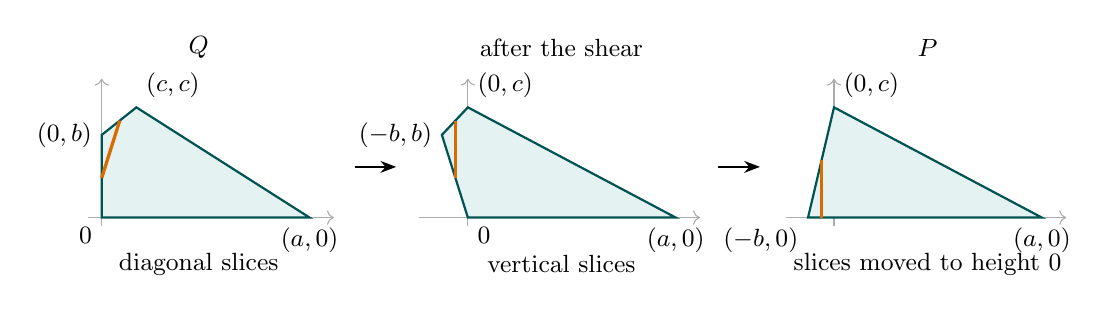
\begin{tikzpicture}[x=.88cm,y=2.8cm,font=\small,
  polyshape/.style={draw=teal!65!black,fill=teal!10,line width=.8pt},
  slice/.style={draw=orange!85!black,line width=1.2pt}]
  \begin{scope}
    \node at (1.4,.77) {$Q$};
    \draw[->,gray!65] (-.2,0)--(3.35,0);
    \draw[->,gray!65] (0,-.04)--(0,.63);
    \path[polyshape] (0,0)--(3,0)--(.5,.5)--(0,.375)--cycle;
    \node[below left] at (0,0) {$0$};
    \node[below] at (3,0) {$(a,0)$};
    \node[above right] at (.5,.5) {$(c,c)$};
    \node[left] at (0,.375) {$(0,b)$};
    \draw[slice] (0,.18)--(.26,.44);
    \node at (1.4,-.21) {diagonal slices};
  \end{scope}
  \begin{scope}[xshift=4.65cm]
    \node at (1.35,.77) {after the shear};
    \draw[->,gray!65] (-.7,0)--(3.35,0);
    \draw[->,gray!65] (0,-.04)--(0,.63);
    \path[polyshape] (0,0)--(3,0)--(0,.5)--(-.375,.375)--cycle;
    \node[below right] at (0,0) {$0$};
    \node[below] at (3,0) {$(a,0)$};
    \node[above right] at (0,.5) {$(0,c)$};
    \node[left] at (-.375,.375) {$(-b,b)$};
    \draw[slice] (-.18,.18)--(-.18,.44);
    \node at (1.35,-.21) {vertical slices};
  \end{scope}
  \begin{scope}[xshift=9.3cm]
    \node at (1.35,.77) {$P$};
    \draw[->,gray!65] (-.7,0)--(3.35,0);
    \draw[->,gray!65] (0,-.04)--(0,.63);
    \path[polyshape] (-.375,0)--(3,0)--(0,.5)--cycle;
    \node[below left] at (-.375,0) {$(-b,0)$};
    \node[below] at (3,0) {$(a,0)$};
    \node[above right] at (0,.5) {$(0,c)$};
    \draw[slice] (-.18,0)--(-.18,.26);
    \node at (1.35,-.21) {slices moved to height $0$};
  \end{scope}
  \draw[-{Stealth[length=2mm]},thick] (3.65,.23)--(4.25,.23);
  \draw[-{Stealth[length=2mm]},thick] (8.9,.23)--(9.5,.23);
\end{tikzpicture}
\caption{Bounding polygons in the diagonal compression.  The shear turns
lines of direction $(1,1)$ into vertical lines.  Moving each vertical slice
to start at height zero produces $P$; the marked slices correspond under
these operations.  These are continuous bounds: actual row exponents are
replaced by possible vanishing orders, not translated point by point.
All three polygons have area $H/2$.  Axis scales are chosen for legibility.}
\label{fig:node-compression}
\end{figure}%
}

\newcommand{\ReshapingCompressionFigure}{%
\begin{figure}[H]
\centering
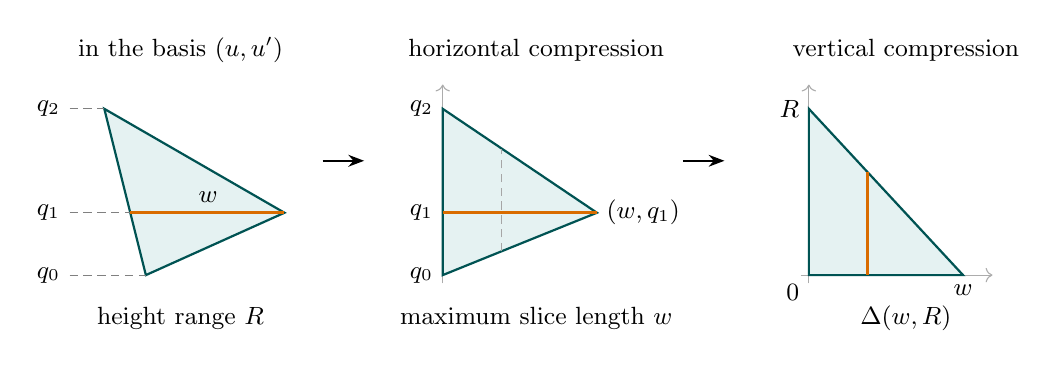
\begin{tikzpicture}[x=.88cm,y=.88cm,font=\small,
  polyshape/.style={draw=teal!65!black,fill=teal!10,line width=.8pt},
  slice/.style={draw=orange!85!black,line width=1.2pt}]
  \begin{scope}
    \node at (1.5,3.25) {in the basis $(u,u')$};
    \path[polyshape] (1,0)--(3,.9)--(.4,2.4)--cycle;
    \draw[densely dashed,gray] (-.1,0)--(1,0);
    \draw[densely dashed,gray] (-.1,.9)--(.775,.9);
    \draw[densely dashed,gray] (-.1,2.4)--(.4,2.4);
    \node[left] at (-.1,0) {$q_0$};
    \node[left] at (-.1,.9) {$q_1$};
    \node[left] at (-.1,2.4) {$q_2$};
    \draw[slice] (.775,.9)--(3,.9);
    \node[above] at (1.9,.9) {$w$};
    \node at (1.5,-.62) {height range $R$};
  \end{scope}
  \begin{scope}[xshift=4.65cm]
    \node at (1.35,3.25) {horizontal compression};
    \draw[->,gray!65] (0,-.12)--(0,2.75);
    \path[polyshape] (0,0)--(2.225,.9)--(0,2.4)--cycle;
    \node[left] at (0,0) {$q_0$};
    \node[left] at (0,.9) {$q_1$};
    \node[left] at (0,2.4) {$q_2$};
    \draw[slice] (0,.9)--(2.225,.9);
    \node[right] at (2.225,.9) {$(w,q_1)$};
    \draw[gray!70,densely dashed] (.85,.344)--(.85,1.827);
    \node at (1.35,-.62) {maximum slice length $w$};
  \end{scope}
  \begin{scope}[xshift=9.3cm]
    \node at (1.4,3.25) {vertical compression};
    \draw[->,gray!65] (-.12,0)--(2.65,0);
    \draw[->,gray!65] (0,-.12)--(0,2.75);
    \path[polyshape] (0,0)--(2.225,0)--(0,2.4)--cycle;
    \node[below left] at (0,0) {$0$};
    \node[below] at (2.225,0) {$w$};
    \node[left] at (0,2.4) {$R$};
    \draw[slice] (.85,0)--(.85,1.483);
    \node at (1.4,-.62) {$\Delta(w,R)$};
  \end{scope}
  \draw[-{Stealth[length=2mm]},thick] (3.55,1.65)--(4.15,1.65);
  \draw[-{Stealth[length=2mm]},thick] (8.75,1.65)--(9.35,1.65);
\end{tikzpicture}
\caption{The primitive direction is chosen so that the transverse height
range is $R=H/w$.  Since the area is $H/2$, the longest horizontal slice
has length $w$.  Horizontal compression aligns the left endpoints of
these slices.  Vertical compression then gives the right triangle with
intercepts $w$ and $R$.  The middle and right panels mark vertical slices
of equal length; the drawing is schematic.}
\label{fig:final-compressions}
\end{figure}%
}


\begin{proof}
Fix the target $w$.  We first use a node to replace the triangular bound
$\Delta(A,B)$ by a quadrilateral of the same area.  A diagonal compression
then produces a triangle with a variable shape.  We choose that shape and a
primitive lattice direction together so that two further compressions give
exactly $\Delta(w,H/w)$.

Throughout, write $\gamma=(\gamma_3,\ldots,\gamma_n)$ for an exponent in
the unchanged coordinates.  For a label occurring in degree $k$, the pair
exponents with this label lie in
\begin{equation}\label{eq:residual-degree}
 \kappa\Delta(A,B),\qquad
 \kappa=k-\sum_{i=3}^n\frac{\gamma_i}{a_i}\ge0.
\end{equation}
For $n=2$ the label is empty and $\kappa=k$.  Each operation below acts on
these two-coordinate spaces, carrying the common monomial with exponent
$\gamma$ along unchanged.  In particular, a planar bound by $\kappa K$
will hold simultaneously for every label.  If $\kappa=0$, the only possible
pair exponent is zero and it stays zero throughout; hence the geometric
calculations may be made with $\kappa>0$.

\paragraph{The node and its exponent bound.}
In pair variables $x,y$, consider
\begin{equation}\label{eq:node-polynomial}
 g(x,y)=y^2-x^2(1+x).
\end{equation}
This polynomial is irreducible, since $1+x$ is not a square in $\C(x)$.
Its curve has the parametrization
\begin{equation}\label{eq:node-parametrization}
 x=v^2-1,\qquad y=v(v^2-1),
\end{equation}
which covers the part where $x\ne0$.  Near the origin choose the analytic
square root with value $1$ and set
\begin{equation}\label{eq:node-coordinates}
 \xi=y+x\sqrt{1+x},\qquad
 \eta=y-x\sqrt{1+x}.
\end{equation}
These are local coordinates and $g=\xi\eta$.

For now fix a real parameter $t>0$, and order the Taylor exponents $(\alpha,\beta)$
in $\xi,\eta$ by lexicographic comparison of
$(\alpha+t\beta,\beta)$, and denote the least exponent by $\nu_t$.
This is a multiplicative well-order: only finitely many nonnegative integer
exponents have weight below any given bound.  The node gives two controls
on these exponents: its two branches bound the least weight after factors
of $g$ have been removed, while each extracted factor translates the least
exponent by $(1,1)$.

Let $f\ne0$ be supported in $\kappa\Delta(A,B)$, and write $f=g^j f_0$,
where $j\ge0$ and $g$ does not divide $f_0$.
The weighted polynomial degree with weights $(1/A,1/B)$ is additive on
nonzero products, since highest-weight forms multiply nontrivially.  As
$g$ has weighted degree $d$, the weighted degree of $f_0$ is at most
$\kappa-jd$, which is nonnegative.  Under
\eqref{eq:node-parametrization}, its restriction is a nonzero polynomial
in $v$: otherwise $f_0$ would vanish on the irreducible curve $g=0$.
Define
\begin{equation}\label{eq:normalization-degree-constant}
 W=\max(2A,3B)=dH.
\end{equation}
The monomial inequality
\[
 2i+3i'\le W\left(\frac{i}{A}+\frac{i'}{B}\right)
\]
shows that the restriction polynomial has degree at most
\begin{equation}\label{eq:restriction-degree}
 (\kappa-jd)W.
\end{equation}

Let $\mu$ be the weight of $\nu_t(f_0)$.  At $v=1$, the branch is
$\eta=0$ and $\xi$ vanishes simply.  At $v=-1$, the branch is $\xi=0$
and $\eta$ vanishes simply.  Indeed, the chosen square root becomes $v$
near $1$ and $-v$ near $-1$, and the nonzero branch coordinate in either
case is $2v(v^2-1)$.  Every nonzero pure $\xi$ term in $f_0$ has exponent
at least $\mu$, and every nonzero pure $\eta$ term has exponent at least
$\mu/t$.  The restriction polynomial therefore has orders at least
$\mu$ and $\mu/t$ at these two distinct points.  Comparing their sum with
\eqref{eq:restriction-degree} gives
\begin{equation}\label{eq:two-branch-bound}
 \left(1+\frac1t\right)\mu\le(\kappa-jd)W.
\end{equation}
To express this bound as a triangle, define its intercepts
\begin{equation}\label{eq:node-intercepts}
 a=\frac{Wt}{1+t},\qquad b=\frac{W}{1+t}.
\end{equation}
For $\nu_t(f_0)=(\alpha,\beta)$, inequality~\eqref{eq:two-branch-bound}
is exactly $\alpha/a+\beta/b\le\kappa-jd$.  Hence
$\nu_t(f_0)\in(\kappa-jd)\Delta(a,b)$.

The extracted factors account for the rest of the degree bound.  Set
$c=1/d$, so their contribution is
$\nu_t(g^j)=(j,j)=jd(c,c)$.  The coefficients $\kappa-jd$ and $jd$
sum to $\kappa$, and therefore
\begin{equation}\label{eq:node-envelope}
 \begin{split}
 \nu_t(f)&\in(\kappa-jd)\Delta(a,b)+jd\{(c,c)\}\subset\kappa Q,\\
 Q&=\conv\{(0,0),(a,0),(c,c),(0,b)\}.
 \end{split}
\end{equation}
Thus the axis triangle comes from the two branch orders, and the diagonal
point comes from powers of the node equation.

From this point on, restrict the free parameter to $t>T$, where
\begin{equation}\label{eq:node-parameters}
 T=d^2H=\max(9B/A,4A/B)\ge6.
\end{equation}
The inequality
\[
 \frac ca+\frac cb=\frac{(1+t)^2}{Tt}>1
\]
shows that $Q$ is a quadrilateral with the vertices in the stated order.
Its area is
\begin{equation}\label{eq:node-area}
 \operatorname{area}(Q)=\frac{c(a+b)}2=\frac H2.
\end{equation}
The identity $W=dH$ is what makes this area equal to that of the input
triangle $\Delta(A,B)$.  The parameter $t$ remains free to change the
shape of $Q$ for the later lattice-direction choice.
For each label, replace its pair support by the possible values of
$\nu_t$ on its polynomial span.  The product of the spaces in degrees
$k,l$ with labels $\gamma,\gamma'$ lies in the space of degree $k+l$
with label $\gamma+\gamma'$, by the original support inclusion.
Lemmas~\ref{lem:least-terms}
and~\ref{lem:row-valuation} preserve cardinality and the graded inclusion,
and \eqref{eq:node-envelope} supplies the bound $\kappa Q$.

We also need the jet implication for this change.  At each fixed degree,
choose a basis with distinct least exponents in each nonempty label space.
One sufficiently small $e>0$ makes weights $(1,t+e)$ select all these
least terms strictly.  To see this, choose $M$ larger than all the selected
$(1,t)$-weights.  Among the finitely many exponents of weight at most $M$,
a small positive perturbation preserves strict comparisons and realizes
the tie-break by the second exponent.  Make $e$ smaller still so that all
selected weights remain below $M$; exponents originally above $M$ cannot
interfere, because a positive perturbation only increases their weights.
Lemmas~\ref{lem:weighted-limit}
and~\ref{lem:rank-transfer} apply under
$(\xi,\eta)=(sX,s^{t+e}Y)$, with the other variables unchanged.
Their inverse images are torus points.  In fact, for each of the finitely
many test points with $X,Y\ne0$, one has $\eta/\xi\to0$, while
\[
 x=\frac{\xi-\eta}{2}+O\bigl((\xi-\eta)^2\bigr),
 \qquad y=\frac{\xi+\eta}{2}.
\]
Thus $x,y\ne0$ for all sufficiently small positive $s$.  The local
coordinate map is injective on a common neighborhood, so it also preserves
distinctness of the test points.

\paragraph{From the quadrilateral to a triangle.}
Apply the integral shear
\[
 (\alpha,\beta)\longmapsto(\alpha-\beta,\beta)
\]
and then compress in the second coordinate.  The transformed quadrilateral
has vertices $(0,0),(a,0),(0,c),(-b,b)$.  For first coordinate $q$ in
$[-b,0]$, its lower boundary is $-q$ and its upper boundary is
$c+(c-b)q/b$; their difference is $c(1+q/b)$.  For $q\in[0,a]$, the
vertical slice length is $c(1-q/a)$.  Compression therefore gives the
triangle
\begin{equation}\label{eq:compressed-triangle}
 P=\conv\{(-b,0),(a,0),(0,c)\},\qquad
 \operatorname{area}(P)=\frac H2.
\end{equation}
Figure~\ref{fig:node-compression} displays these slice lengths geometrically.
Lemmas~\ref{lem:unimodular} and~\ref{lem:compression} show that the exponent
sets remain graded, retain their cardinalities, admit backward jet
transfer, and are bounded, label by label, by $\kappa P$.

\ReshapingNodeFigure

The area is now correct, but we have not yet obtained the prescribed
intercept $w$.  We choose a primitive integral direction whose transverse
range is exactly $H/w$.  In the resulting coordinates, the longest
horizontal slice will have length $w$; compression will turn that length
into the horizontal intercept.

\paragraph{Choosing the primitive direction.}
Put $R=H/w$ and $a_0=WT/(1+T)$.  As $t$ ranges over $(T,\infty)$,
the intercept $a$ ranges over $(a_0,W)$.  Choose $j$ to be the largest
power of two not exceeding
\[
 \frac{R}{2W}=\frac{1}{2dw}.
\]
Then
\begin{equation}\label{eq:primitive-j}
 j>\frac{1}{4dw}>4,
 \qquad R-jW\ge\frac R2>0.
\end{equation}
The open interval
\begin{equation}\label{eq:primitive-interval}
 \bigl(d(R-jW),\ d(R-ja_0)\bigr)
\end{equation}
has length
\[
 \frac{djW}{1+T}=\frac{jT}{1+T}>2.
\]
It therefore contains an odd integer $i$.  This is the point of choosing
$j$ to be a power of two: the vector $u=(i,j)$ is automatically primitive.
Choose the unique $t>T$ for which
\begin{equation}\label{eq:tuned-intercept}
 a=\frac{R-i/d}{j}.
\end{equation}
The interval \eqref{eq:primitive-interval} ensures that this value lies in
$(a_0,W)$.

At the three vertices $(-b,0),(a,0),(0,c)$ of $P$, the functional
$z\mapsto\det(u,z)$ takes values $jb,-ja,i/d$, respectively.  They are
distinct and ordered as
\begin{equation}\label{eq:vertex-heights}
 -ja<jb<i/d,
 \qquad i/d-jb=R-jW>0.
\end{equation}
Their range is exactly $i/d+ja=R$.  This choice used only inequalities
between real numbers; in particular, no rationality of the intercepts was
required.  We now fix this $t$ and this primitive vector for all degrees.

\paragraph{The two final compressions.}
Complete $u$ to an integral basis $(u,u')$ with determinant $1$, and use
the coefficients in that basis as new exponent coordinates.  The second
coordinate of a vector $z$ is $\det(u,z)$.  Thus the transformed triangle
still has area $H/2$, and its three vertex heights, say
$q_0<q_1<q_2$, satisfy $q_2-q_0=R$.

Its horizontal slice length is zero at $q_0$, increases linearly up to
$q_1$, and decreases linearly to zero at $q_2$.  If the maximum slice
length is $h_{\max}$, integration of this tent gives area
$Rh_{\max}/2$.  Hence $h_{\max}=H/R=w$.  Compressing in the first
coordinate therefore gives
\begin{equation}\label{eq:tent-triangle}
 \conv\{(0,q_0),(w,q_1),(0,q_2)\}.
\end{equation}
Its vertical slice at first coordinate $h\in[0,w]$ has length
$R(1-h/w)$.  A final compression in the second coordinate produces
$\Delta(w,R)$, as illustrated in Figure~\ref{fig:final-compressions}.

\ReshapingCompressionFigure

All these changes satisfy Lemmas~\ref{lem:unimodular}
and~\ref{lem:compression}.  They commute with scaling of the bounding
shapes, so for the label $\gamma$ the final pair exponents lie in
$\kappa\Delta(w,R)$.  Substituting \eqref{eq:residual-degree} gives
\eqref{eq:reshape-bound}.  Cardinality, the graded inclusion, and the
backward jet implication hold at every stage, proving all the assertions.

For clarity, the sets in every degree are defined by the fixed exact order
$\nu_t$, the fixed integral maps, and exact orders of vanishing at $1$.
The perturbation $e$ and the small scaling parameters only witness
jet-rank implications at a specified degree.  They may depend on that
degree and on the test tuple without changing the sets or their graded
inclusion.
\end{proof}

\section{Interior lattice points and interpolation}
\label{sec:saturation}

The reshaping proposition preserves the number of monomials, but does not
describe each resulting exponent. For interpolation we need more than the
correct asymptotic number: we need specific sets of exponents. Additivity
across degrees supplies the missing information. An additive family $F_k$
occupying asymptotically the full volume of $kP$ contains every lattice point
of $kK$ for each fixed compact set $K\subset\operatorname{int}P$, once the
degree $k$ is sufficiently large.

The general semigroup approximation theorem of
\citet[Theorem~1.6]{KavehKhovanskii2012} provides a broader setting for
interior-saturation statements. Under the full-density hypothesis needed
here, the following direct proof uses only decompositions into two summands.

\begin{lemma}[Interior saturation]
\label{lem:interior-saturation}
Let $n\ge1$ be an integer, let $P\subset\R^n$ be a compact convex set with
nonempty interior, and let $F_k\subset kP\cap\Z^n$ for every integer
$k\ge1$. Suppose that
\[
 F_k+F_l\subset F_{k+l}\quad(k,l\ge1),
 \qquad
 \#F_k=\vol(P)k^n+o(k^n).
\]
For every compact set $K\subset\operatorname{int}P$, there is an integer
$k_K$ such that
\[
 kK\cap\Z^n\subset F_k\qquad(k\ge k_K).
\]
\end{lemma}

\begin{proof}
The lattice-point estimate for a full-dimensional compact convex set gives
\[
 \#(kP\cap\Z^n)=\vol(P)k^n+o(k^n).
\]
Consequently the sets of missing exponents
\[
 H_k=(kP\cap\Z^n)\setminus F_k
\]
satisfy $\#H_k=o(k^n)$. This estimate alone would allow individual missing
points deep inside $kP$. We use additivity to exclude them.

We may assume that $K$ is nonempty. Choose $\delta>0$ so that every closed
ball of radius $\delta$ centered in $K$ is contained in $P$. For a large
integer $k$, put $k_1=\lfloor k/2\rfloor$ and $k_2=k-k_1$, and fix
$y\in kK\cap\Z^n$. Write $z=y/k$. Every integer vector $y_1$ satisfying
\[
 \lVert y_1-k_1z\rVert\le\delta\min(k_1,k_2)
\]
gives a decomposition $y=y_1+y_2$ with $y_i\in k_iP\cap\Z^n$. Indeed,
both $y_1/k_1$ and $y_2/k_2$ are within distance $\delta$ of $z$.
The ball in this display contains at least $c k^n$ lattice points for all
sufficiently large $k$, where $c>0$ is independent of $y$.

At most $\#H_{k_1}$ choices have $y_1\notin F_{k_1}$, and at most
$\#H_{k_2}$ choices have $y_2\notin F_{k_2}$, because $y_1\mapsto y-y_1$
is injective. The total number excluded is $o(k^n)$. Thus some decomposition
has $y_i\in F_{k_i}$, and additivity gives $y\in F_k$. All constants and
degree thresholds used here are uniform over $y\in kK\cap\Z^n$.
\end{proof}

The lemma requires no finite-generation hypothesis on the sets $F_k$ or on
the semigroup they form. It also permits real, rather than rational,
bounding polytopes. We next describe the exponents needed for interpolation
in the simplex that will result from repeated reshaping.

\begin{lemma}[Interpolation in an elongated simplex]
\label{lem:simplex-interpolation}
Let $n\ge2$, $r\ge1$, and $m\ge0$ be integers, and let
$c_1,\ldots,c_r\in\C^*$ be distinct. Put
\[
 E_{r,m}=
 \left\{(\beta,b)\in\Z_{\ge0}^{n-1}\times\Z_{\ge0}:
       |\beta|+\frac br<m+1\right\}.
\]
Then $\M(E_{r,m})$ surjects onto jets through degree $m$ at the points
\[
 q_i=(1,\ldots,1,c_i)\in\Torus^n,\qquad 1\le i\le r.
\]
\end{lemma}

\begin{proof}
Write the coordinates as $(x',Y)$, with $n-1$ coordinates in $x'$. At $q_i$,
an arbitrary jet through degree $m$ has a unique expression
\[
 \sum_{|\alpha|\le m}(x'-1)^\alpha h_{i,\alpha}(Y-c_i),
 \qquad
 \deg h_{i,\alpha}\le m-|\alpha|.
\]
For each $\alpha$, the Chinese remainder theorem provides a polynomial
$f_\alpha(Y)$ such that
\[
 \begin{split}
 f_\alpha(Y)&\equiv h_{i,\alpha}(Y-c_i)
       \pmod{(Y-c_i)^{m+1-|\alpha|}}\quad(1\le i\le r),\\
 \deg f_\alpha&<r(m+1-|\alpha|).
 \end{split}
\]
The polynomial
\[
 f(x',Y)=\sum_{|\alpha|\le m}(x'-1)^\alpha f_\alpha(Y)
\]
has all the prescribed jets. Every monomial $(x')^\beta Y^b$ occurring in
its $\alpha$-summand satisfies $\beta\le\alpha$ componentwise and hence
\[
 |\beta|+\frac br
 \le |\alpha|+\frac br
 <|\alpha|+(m+1-|\alpha|)=m+1.
\]
Thus $f\in\M(E_{r,m})$.
\end{proof}

The two lemmas now convert asymptotically full additive supports into
simultaneous jet surjectivity. Translating a slightly smaller simplex into
the interior avoids any assertion about exponents on the boundary.

\begin{proposition}[Jets from full-volume supports]
\label{prop:asymptotic-jets}
Let $n\ge2$ and $r\ge1$ be integers, let $w>0$, and set
\[
 P=\Delta(w,\ldots,w,rw).
\]
Suppose that finite sets $F_k\subset kP\cap\Z^n$, indexed by all integers
$k\ge1$, satisfy
\[
 F_k+F_l\subset F_{k+l},
 \qquad
 \#F_k=\vol(P)k^n+o(k^n).
\]
For every $0<\theta<w$ and every choice of distinct
$c_1,\ldots,c_r\in\C^*$, the space $\M(F_k)$ surjects onto jets through
degree $\lfloor k\theta\rfloor$ at $(1,\ldots,1,c_i)$ for all sufficiently
large $k$.
\end{proposition}

\begin{proof}
Choose $\theta/w<\lambda<1$. There is a vector $a$ with strictly positive
coordinates such that $a+\lambda P\subset\operatorname{int}P$: it suffices
to require
\[
 \frac{a_1+\cdots+a_{n-1}}w+\frac{a_n}{rw}<1-\lambda.
\]
Choose $a_k\in k^{-1}\Z^n$ with $a_k\to a$. For all sufficiently large
$k$, the translated simplices $a_k+\lambda P$ lie in a single compact
subset $K$ of $\operatorname{int}P$. Lemma~\ref{lem:interior-saturation}
therefore gives
\[
 ka_k+(k\lambda P\cap\Z^n)\subset F_k.
\]
Consequently $\M(F_k)$ contains the monomial space for
$k\lambda P\cap\Z^n$, multiplied by the monomial with exponent $ka_k$.
Multiplication by this monomial is an isomorphism on each jet algebra at
a torus point, since the monomial is a unit there.

Put $m=\lfloor k\theta\rfloor$. For all sufficiently large $k$,
$m+1\le k\lambda w$, and hence
\[
 E_{r,m}\subset k\lambda P\cap\Z^n.
\]
Lemma~\ref{lem:simplex-interpolation} supplies jet surjectivity for this
subspace. The monomial translation preserves surjectivity and proves the
claim.
\end{proof}

\section{Proof of the main theorem}
\label{sec:conclusion}

We now assemble the exponent construction and interpolation results. The
reshaping parameters will depend on the point count $r$, but a single
threshold will allow every sufficiently large integer $r$. The final
passage from jets to intersection numbers uses ordinary curve
multiplicities, including at singular points of the curves.

\subsection{The exponent sets for every sufficiently large point count}

Fix the polarized variety $(X,L)$ of Theorem~\ref{thm:main}, and write
$V=L^n$. Choose an integer $D>0$ for which $DL$ is very ample.
Proposition~\ref{prop:flag-simplex} supplies additive support sets $S_k$ with
\[
 S_k\subset kP_0\cap\Z^n,
 \qquad
 \#S_k=h^0(X,kL).
\]
Here $P_0=\Delta(1/D,\ldots,1/D,D^{n-1}V)$.
Let $\ell>0$ be the smallest intercept of $P_0$. Choose an integer $r_0$
such that
\begin{equation}
 \label{eq:threshold}
 (V/r)^{1/n}<\ell/100\qquad(r\ge r_0).
\end{equation}
Such a choice exists because $X$ and $L$ are fixed.

Fix any integer $r\ge r_0$, and put $w=(V/r)^{1/n}$. Apply
Proposition~\ref{prop:reshape} to the first two intercepts, replacing them
by $w$ and their product divided by $w$. Keep the intercept $w$ fixed, and
pair the other new intercept with the next untouched one. Continue until
$n-1$ intercepts equal $w$.

Every pair of input intercepts $A,B$ in this procedure satisfies
$A,B\ge\ell$. Indeed, an untouched intercept has this property, and the
new carried intercept $AB/w$ is greater than $A$, since $B\ge\ell>w$.
Thus the hypothesis of Proposition~\ref{prop:reshape} holds at every step:
\[
 w\max(3/A,2/B)\le\frac{3w}{\ell}<\frac1{16}.
\]
The product of all intercepts remains $V$. We obtain finite sets $F_k$ in
\begin{equation}
 \label{eq:final-simplex}
 kP_*,\qquad
 P_* =\Delta(w,\ldots,w,V/w^{n-1})
     =\Delta(w,\ldots,w,rw),
\end{equation}
with
\[
 F_k+F_l\subset F_{k+l},
 \qquad
 \#F_k=h^0(X,kL)=\frac{V}{n!}k^n+o(k^n).
\]
Since $\vol(P_*)=V/n!$, these sets satisfy the hypotheses of
Proposition~\ref{prop:asymptotic-jets}.

For each $0<\theta<w$ and all sufficiently large $k$, that proposition
gives simultaneous jets through degree $\lfloor k\theta\rfloor$ for
$\M(F_k)$ at an $r$-tuple of distinct torus points. Each application of
Proposition~\ref{prop:reshape} transfers this surjectivity to the preceding
support set. Proposition~\ref{prop:flag-simplex} finally transfers it to
$H^0(X,kL)$ at some tuple of distinct points of $X$. In particular, for
every such $\theta$ and $k$, the set
\begin{equation}
 \label{eq:surjectivity-locus}
 \left\{\mathbf p\in U_r(X):
 H^0(X,kL)\longrightarrow
 \bigoplus_{i=1}^r\Jet_{p_i}^{\lfloor k\theta\rfloor}(kL)
 \text{ is surjective}\right\}
\end{equation}
is nonempty. The tuple witnessing this assertion may depend on both
$\theta$ and $k$.

\subsection{A common very-general locus}

For fixed integers $k\ge1$ and $m\ge0$, the locus of tuples at which
$H^0(X,kL)$ surjects onto jets through degree $m$ is Zariski open in
$U_r(X)$. Indeed, the bundle of principal parts of order $m$ of $kL$ is
locally free because $X$ is smooth. Pulling it back along each coordinate
projection of $U_r(X)$ gives an algebraic vector-bundle map
\[
 H^0(X,kL)\otimes\mathcal O_{U_r(X)}
 \longrightarrow
 \bigoplus_{i=1}^r\operatorname{pr}_i^*\mathcal P^m(kL).
\]
Its surjectivity locus is defined by the nonvanishing of maximal minors.

Choose $0<\theta_j<w$ with $\theta_j\uparrow w$. For each $j$, choose
$k_j$ so that the locus in \eqref{eq:surjectivity-locus} is nonempty and
$\lfloor k\theta_j\rfloor\ge1$ for every $k\ge k_j$. Denote this open
locus by $O_{j,k}$ and set
\begin{equation}
 \label{eq:exceptional-set}
 Z_r=\bigcup_{j\ge1}\ \bigcup_{k\ge k_j}
       \bigl(U_r(X)\setminus O_{j,k}\bigr).
\end{equation}
Every set in this countable union is a proper Zariski-closed subset of
$U_r(X)$.

The complement is nonempty. The complex points of $U_r(X)$ form a
nonempty locally compact Hausdorff space, and hence a Baire space. Since
$U_r(X)$ is smooth and irreducible, every proper algebraic closed subset
has empty interior in its complex topology. A countable union of these
closed subsets cannot cover $U_r(X)$. Thus every tuple outside $Z_r$
simultaneously has all the jet-surjectivity properties indexed by $j$ and
$k\ge k_j$.

\subsection{From jets to ordinary curve multiplicities}

The relation between Seshadri constants and jet separation appears in
Demailly's one-point formulation \cite[Section~6]{Demailly1992} and in the
weighted multipoint framework of \citet[Section~5]{Ito2013}. The following elementary
implication is the one needed here. We give its local proof, including at
singular points of the curves.

\begin{lemma}[Jets bound curve intersections]
\label{lem:jets-curves}
Let $X$ be a smooth complex projective variety, let $A$ be a line bundle
on $X$, and let $p_1,\ldots,p_r$ be distinct points. Suppose that, for an
integer $m\ge1$, the map
\[
 H^0(X,A)\longrightarrow\bigoplus_{i=1}^r\Jet_{p_i}^{m}(A)
\]
is surjective. Then every integral curve $C\subset X$ satisfies
\[
 A\cdot C\ge m\sum_{i=1}^r\mult_{p_i}C
\]
provided that $C$ meets at least one of the points.
\end{lemma}

\begin{proof}
Choose a point $p_i\in C$. The local ring $R=\mathcal O_{C,p_i}$ is a
one-dimensional Noetherian local domain. Its maximal ideal $\frakm_R$
satisfies
\[
 \frakm_R^m/\frakm_R^{m+1}\ne0.
\]
Otherwise Nakayama's lemma would give $\frakm_R^m=0$, contrary to
$\dim R=1$. The quotient map from the ambient local ring to $R$ lifts a
nonzero element of this quotient to a jet on $X$ with no terms of degree
less than $m$. Prescribe this jet at $p_i$ and the zero jet at every other
marked point. By surjectivity, a section $s\in H^0(X,A)$ has these jets.
It vanishes to order at least $m$ at every marked point, and its restriction
to $C$ is nonzero.

We recall the local intersection bound for this restriction. In a
one-dimensional Noetherian local domain $(R,\frakm_R)$, let
$0\ne f\in\frakm_R^m$. For every integer $q\ge1$, multiplication by
powers of $f$ gives
\[
 \length(R/(f^q))=q\,\length(R/(f)).
\]
Since $(f^q)\subset\frakm_R^{mq}$, the Hilbert--Samuel formula yields
\[
 q\,\length(R/(f))
 \ge\length(R/\frakm_R^{mq})
 =mq\,e(R)+O(1),
\]
where $e(R)$ is the ordinary multiplicity. Dividing by $q$ and letting
$q\to\infty$ gives
\begin{equation}
 \label{eq:local-curve-bound}
 \length(R/(f))\ge m\,e(R).
\end{equation}

Apply \eqref{eq:local-curve-bound} to the local equations of $s|_C$ at
the marked points on $C$. The zero scheme of this nonzero section is an
effective Cartier divisor on the integral projective curve, and its total
length is $\deg(A|_C)=A\cdot C$. Summing the local contributions proves
the assertion.
\end{proof}

Fix a tuple $\mathbf p\in U_r(X)\setminus Z_r$. Applying
Lemma~\ref{lem:jets-curves} with $A=kL$ and
$m=\lfloor k\theta_j\rfloor$ gives
\[
 \eps(X,L;\mathbf p)\ge\frac{\lfloor k\theta_j\rfloor}{k}
 \qquad(k\ge k_j).
\]
First let $k\to\infty$ for each fixed $j$, and then let $j\to\infty$.
We obtain
\begin{equation}
 \label{eq:main-lower-bound}
 \eps(X,L;\mathbf p)\ge w=(V/r)^{1/n}.
\end{equation}

\subsection{The volume bound}

For completeness, we derive the reverse inequality for every tuple of
distinct points. Let $\pi:Y\to X$ be the blow-up of such a tuple, with
exceptional divisors $E_1,\ldots,E_r$. For $t\ge0$, put
\[
 D_t=\pi^*L-t\sum_{i=1}^r E_i.
\]
If an integral curve $\Gamma$ is contained in $E_i\simeq\mathbb P^{n-1}$,
then $D_t|_{E_i}=t\mathcal O_{\mathbb P^{n-1}}(1)$ is nonnegative on
$\Gamma$. Every other integral curve is the strict transform of an
integral curve $C\subset X$, and
\begin{equation}
 \label{eq:strict-transform-intersection}
 D_t\cdot\Gamma=L\cdot C-t\sum_{i=1}^r\mult_{p_i}C.
\end{equation}
Here $E_i\cdot\Gamma=\mult_{p_i}C$ also when $C$ is singular. If
$p_i\notin C$, both sides vanish. For $p_i\in C$, identify the strict
transform locally with the blow-up of $\mathcal O_{C,p_i}$ at its maximal
ideal. Its intersection
with $E_i$ is the zero-dimensional exceptional fiber
$\operatorname{Proj}(\operatorname{gr}_{\frakm}\mathcal O_{C,p_i})$,
whose length is the Hilbert--Samuel multiplicity. This is the degree of
the effective Cartier divisor cut out by $E_i$ on the strict transform.

It follows from \eqref{eq:strict-transform-intersection} that $D_t$ is
nef whenever $0\le t<\eps(X,L;\mathbf p)$. A nef real divisor has
nonnegative top self-intersection. The exceptional divisors are disjoint,
$\pi^*L|_{E_i}$ is trivial, and $E_i^n=(-1)^{n-1}$. Therefore
\[
 0\le D_t^n=V-rt^n.
\]
This inequality for all $0\le t<\eps(X,L;\mathbf p)$ proves the universal
bound
\begin{equation}
 \label{eq:volume-upper-bound}
 \eps(X,L;\mathbf p)\le(V/r)^{1/n}.
\end{equation}
Together, \eqref{eq:main-lower-bound} and \eqref{eq:volume-upper-bound}
give the equality asserted in Theorem~\ref{thm:main} at every tuple outside
$Z_r$. Equation~\eqref{eq:strict-transform-intersection} also shows that
$D_w$ is nef there, and its top self-intersection is zero. The threshold
\eqref{eq:threshold} was chosen before fixing $r$, so this proves the
theorem for every integer $r\ge r_0$.

\bibliographystyle{plainnat}
\bibliography{references}
\end{document}
